\documentclass[class=report, crop=false, 12pt,a4paper]{standalone}
\usepackage{enumitem}
\usepackage{float}
\usepackage[normalem]{ulem}
\usepackage{graphicx}
\usepackage{amsmath}
\usepackage{amssymb}
\usepackage{siunitx}
\usepackage{commath}
\usepackage{tikz}
\usetikzlibrary{positioning, fit, calc}   
\tikzset{block/.style={draw, thick, text width=3cm ,minimum height=1.3cm, align=center},   
line/.style={-latex}     
}  
\begin{document}
\section{Constitutive equations}
We want to find a way to link the stress tensor $\tau$ with the velocity field i.e. $\tau = f(u, \ v, \ w)$.
\begin{figure}[H]
  \centering
  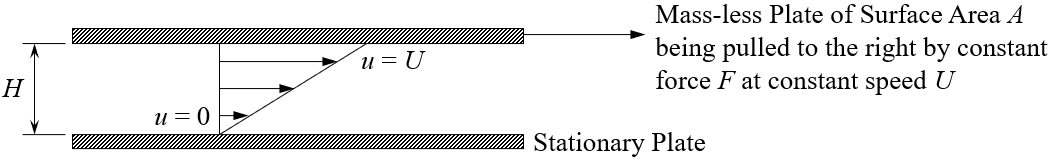
\includegraphics[width = 0.8\textwidth]{../img/diagram1.png}
\end{figure}
The angle of deformation $\Delta \theta$ can be used to derive the following:
\begin{gather}
  \tan{\Delta \theta} = \frac{u \cdot \Delta T}{H}\\
  \tan{\Delta \theta} = \dif \theta = \frac{u\cdot t}{H} \rightarrow \frac{\dif \theta}{\dif t} = \frac{u}{H}\\
  \tau = \frac{F}{A} \propto \frac{\dif \theta}{\dif t} = \frac{u}{H}\\
  \tau = \mu \frac{\dif \theta}{\dif t} = \mu \frac{u}{H}\\
  \tau = \mu \frac{\dif u}{\dif y}
\end{gather}
\begin{itemize}
  \item $\tau$ is the shear stress
  \item $\frac{\dif u}{\dif y}$ is the shear rate
  \item $\mu$ is the dynamic viscosity and has units \si{\newton\second\per\meter\squared}
  \item $\nu = \frac{\mu}{\rho}$ is the kinematic viscosity and has units \si{\meter\squared\per\second}
\end{itemize}
For Newtonian fluids, $\mu$ is constant. In the case above, our stress tensor is $\tau_{yx}$, hence:
\begin{equation}
  \tau_{yx} = \mu \frac{\partial u}{\partial y}
\end{equation}
Our velocity gradient can be defined as:
\begin{equation}
  \nabla \vec{V} = \begin{bmatrix}
    \frac{\partial u}{\partial x} & \frac{\partial v}{\partial x} & \frac{\partial w}{\partial x}\\
    \frac{\partial u}{\partial y} & \frac{\partial v}{\partial y} & \frac{\partial w}{\partial y}\\
    \frac{\partial u}{\partial z} & \frac{\partial v}{\partial z} & \frac{\partial w}{\partial z}
  \end{bmatrix}
\end{equation}
The left diagonal components are the normal deformation, orthogonal to the surface.
\begin{figure}[H]
  \centering
  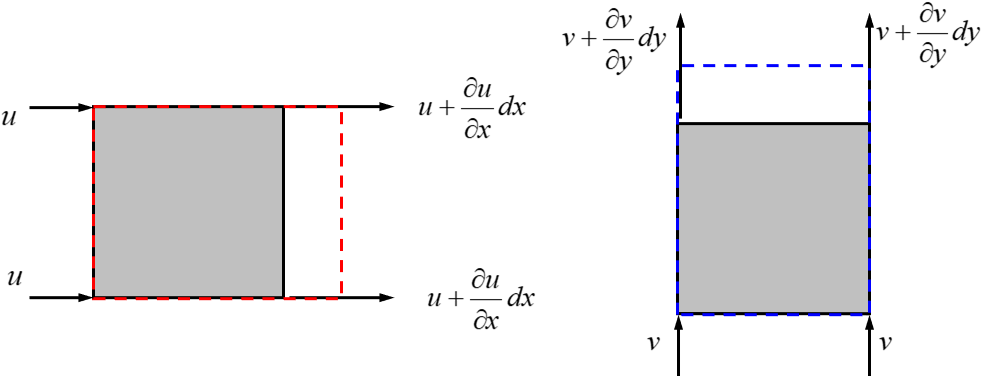
\includegraphics[width = 0.8\textwidth]{../img/diagram2.png}
\end{figure}
A simplified way of writing these left diagonal terms is
\begin{equation}
  \nabla \cdot \vec{V} = \frac{\partial u_i}{\partial x_i} = \frac{\partial u}{\partial x} + \frac{\partial v}{\partial y} + \frac{\partial w}{\partial z} 
\end{equation}
The repeated index $i$ means sum in the x, y and z directions.
\begin{figure}[H]
  \centering
  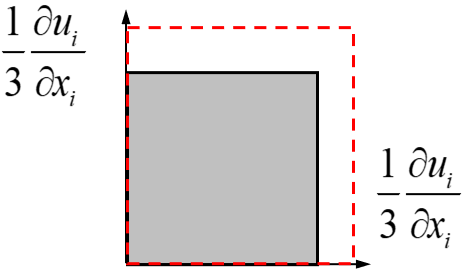
\includegraphics[width = 0.5\textwidth]{../img/diagram3.png}
  \caption{$1/3$ symbolises the average deformation in x, y and z.}
\end{figure}
To find $\frac{\partial u}{\partial x}$, we can do the following
\begin{equation}
  \frac{\partial u}{\partial x} = \frac{1}{3}\frac{\partial u_i}{\partial x_i} + \left( \frac{\partial u}{\partial x} - \frac{1}{3}\frac{\partial u_i}{\partial x_i} \right)
\end{equation}
\begin{figure}[H]
  \centering
  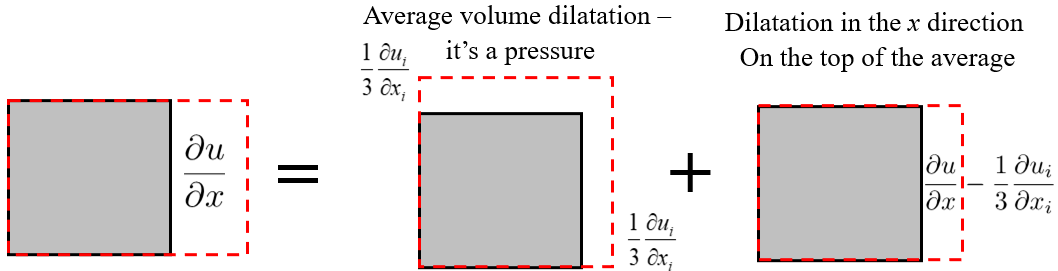
\includegraphics[width = \textwidth]{../img/diagram4.png}
\end{figure}
This can be also done for the other two orthogonal directions
\begin{gather}
  \frac{\partial v}{\partial y} = \frac{1}{3}\frac{\partial u_i}{\partial x_i} + \left( \frac{\partial v}{\partial y} - \frac{1}{3}\frac{\partial u_i}{\partial x_i} \right)\\
  \frac{\partial w}{\partial z} = \frac{1}{3}\frac{\partial u_i}{\partial x_i} + \left( \frac{\partial w}{\partial z} - \frac{1}{3}\frac{\partial u_i}{\partial x_i} \right)
\end{gather}
Let us consider another term, such as $\frac{\partial u}{\partial y}$. We can define this as a component of deformation and rotation of the fluid particle.
\begin{equation}
  \frac{\partial u}{\partial y}=\frac{1}{2} \left(\frac{\partial u}{\partial y} + \frac{\partial v}{\partial x}\right) + \left(\frac{\partial u}{\partial y} - \frac{\partial v}{\partial x}\right)
\end{equation}
\begin{figure}[H]
  \centering
  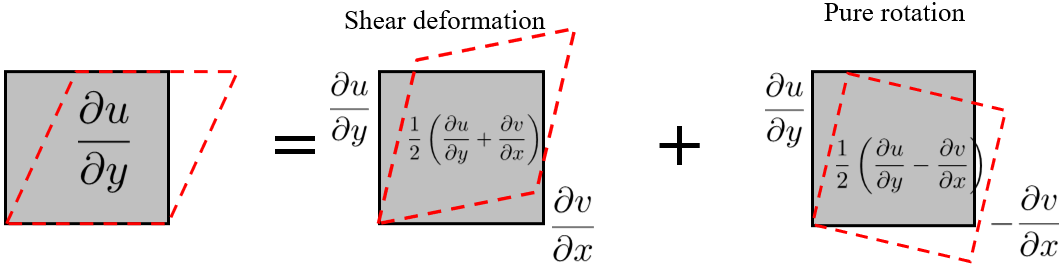
\includegraphics[width = \textwidth]{../img/diagram5.png}
\end{figure}
\subsubsection{Example}
\begin{gather}
  \frac{\partial u}{\partial y}=3=\frac{1}{2} \left(\frac{\partial u}{\partial y} + \frac{\partial v}{\partial x}\right) + \left(\frac{\partial u}{\partial y} - \frac{\partial v}{\partial x}\right) = 2.5 + 0.5\\
  \frac{\partial v}{\partial x}=2=\frac{1}{2} \left(\frac{\partial u}{\partial y} + \frac{\partial v}{\partial x}\right) + \left(\frac{\partial v}{\partial x} - \frac{\partial u}{\partial y}\right) = 2.5 - 0.5
\end{gather}
\begin{figure}[H]
  \centering
  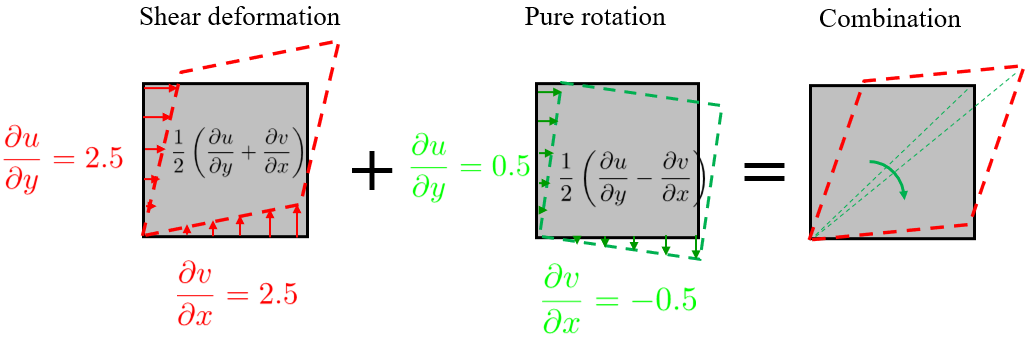
\includegraphics[width = \textwidth]{../img/diagram6.png}
\end{figure}
\begin{figure}[H]
  \centering
  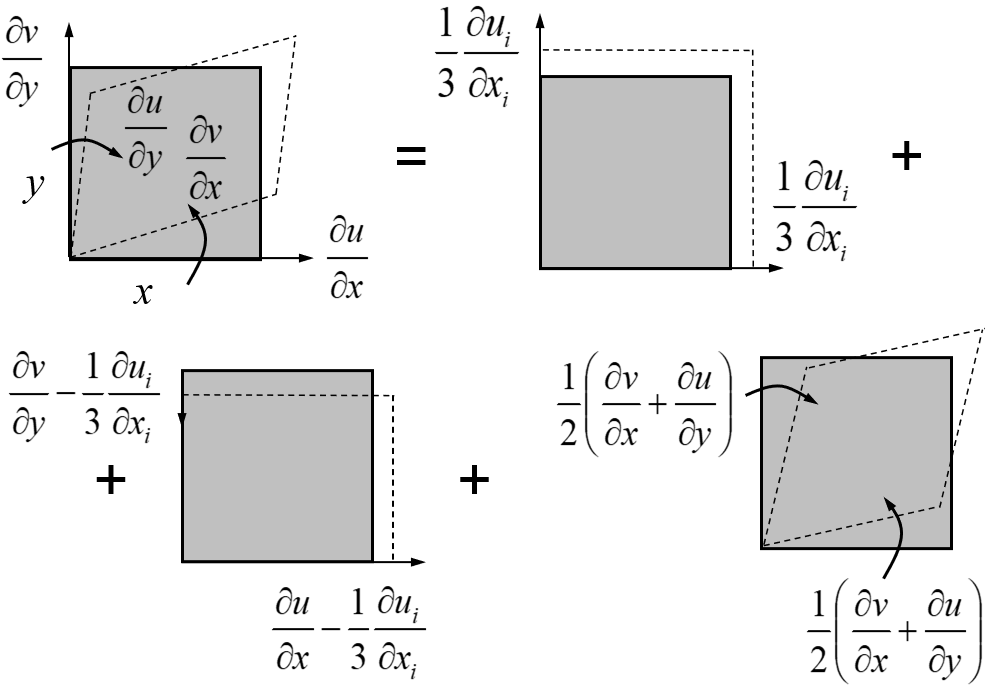
\includegraphics[width = 0.8 \textwidth]{../img/diagram7.png}
\end{figure}
\subsection{Strain rate tensor}
\begin{equation}
  s = \begin{bmatrix}
    \frac{\partial u}{\partial x} & \frac{1}{2} \left[ \frac{\partial u}{\partial y} + \frac{1}{2} \frac{\partial v}{\partial x} \right] & \left[ \frac{\partial u}{\partial z} + \frac{\partial w}{\partial x} \right]\\
    \frac{1}{2} \left[ \frac{\partial u}{\partial y} + \frac{\partial v}{\partial x} \right] & \frac{\partial v}{\partial y} & \frac{1}{2} \left[ \frac{\partial v}{\partial z} + \frac{\partial w}{\partial y} \right] \\
    \frac{1}{2} \left[ \frac{\partial u}{\partial z} + \frac{\partial w}{\partial x} \right] & \frac{1}{2} \left[ \frac{\partial v}{\partial z} + \frac{\partial w}{\partial y} \right] & \frac{\partial w}{\partial z}
  \end{bmatrix} =
\end{equation}
\begin{multline}
  \begin{bmatrix}
    \frac{1}{3} \nabla \cdot \vec{V} & 0 & 0\\
    0 & \frac{1}{3} \nabla \cdot \vec{V} & 0\\
    0 & 0 & \frac{1}{3} \nabla \cdot \vec{V}\\ 
  \end{bmatrix} + \\
  \begin{bmatrix}
    \left[\frac{\partial u}{\partial x} - \frac{1}{3} \nabla \cdot \vec{V} \right] & \frac{1}{2} \left[ \frac{\partial u}{\partial y} + \frac{1}{2} \frac{\partial v}{\partial x} \right] & \frac{1}{2} \left[ \frac{\partial u}{\partial z} + \frac{\partial w}{\partial x} \right]\\
    \frac{1}{2} \left[ \frac{\partial u}{\partial y} + \frac{\partial v}{\partial x} \right] & \left[ \frac{\partial v}{\partial y} - \frac{1}{3} \nabla \cdot \vec{V} \right] & \frac{1}{2} \left[ \frac{\partial v}{\partial z} + \frac{\partial w}{\partial y} \right] \\
    \frac{1}{2} \left[ \frac{\partial u}{\partial z} + \frac{\partial w}{\partial x} \right] & \frac{1}{2} \left[ \frac{\partial v}{\partial z} + \frac{\partial w}{\partial y} \right] & \left[ \frac{\partial w}{\partial z} - \frac{1}{3} \nabla \cdot \vec{V} \right]
  \end{bmatrix}
\end{multline}
\begin{multline}
  \textrm{Deformation part which goes in pressure } \rho \ +\\ \textrm{Deformation part which goes in the stress tensor } T
\end{multline}
Compact notation of the strain rate tensor, indices $i, \ j = 1, \ 2,\ 3$
\begin{equation}
  s_{ij} = \frac{1}{2} \left( \frac{\partial u_i}{\partial x_j} + \frac{\partial u_j}{\partial x_i} \right)
\end{equation}
\subsection{Stress tensor}
\begin{gather}
  T = \begin{bmatrix}
    \tau_xx & \tau_yx & \tau_zx\\
    \tau_xy & \tau_yy & \tau_zy\\
    \tau_xz & \tau_yz & \tau_zz
  \end{bmatrix} = \\ 
  \begin{bmatrix}
    \mu \left[ 2 \frac{\partial u}{\partial x} - \frac{2}{3} \nabla \cdot \vec{V} \right] & \mu \left[ \frac{\partial u}{\partial y} + \frac{1}{2} \frac{\partial v}{\partial x} \right] & \mu \left[ \frac{\partial u}{\partial z} + \frac{\partial w}{\partial x} \right]\\
    \mu \left[ \frac{\partial u}{\partial y} + \frac{\partial v}{\partial x} \right] & \mu\left[ 2\frac{\partial v}{\partial y} - \frac{2}{3}\nabla \cdot \vec{V} \right] & \mu \left[ \frac{\partial v}{\partial z} + \frac{\partial w}{\partial y} \right] \\
    \mu \left[ \frac{\partial u}{\partial z} + \frac{\partial w}{\partial x} \right] & \mu \left[ \frac{\partial v}{\partial z} + \frac{\partial w}{\partial y} \right] & \mu \left[ 2\frac{\partial w}{\partial z} - \frac{2}{3}\nabla \cdot \vec{V} \right]
  \end{bmatrix}
\end{gather}
Compact notation for constitutive equation:
\begin{gather}
  \tau_{ij} = 2\mu \left[ s_{ij} - \frac{1}{3}(\nabla \cdot \vec{V}) \delta_{ij} \right] = \mu \left[ \left(\frac{\partial u_i}{\partial x_j} + \frac{\partial u_j}{\partial x_i} \right) - \frac{2}{3}(\nabla \cdot \vec{V}) \delta_{ij} \right]\\
  \delta_{ij} = \begin{cases}
    1 \textrm{ if } i = j\\
    0 \textrm{ if } i \neq j
  \end{cases} 
\end{gather}
The stress tensor is always symmetric along the left diagonal.
\begin{figure}[H]
  \centering
  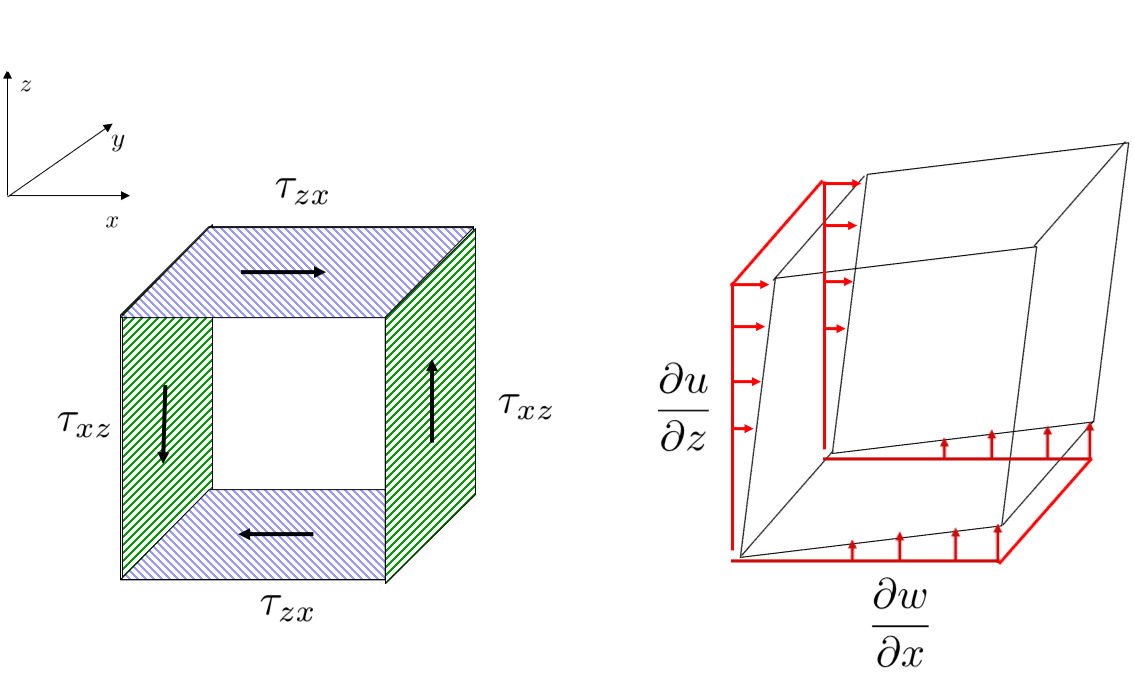
\includegraphics[width = 0.8\textwidth]{../img/diagram8.png}
\end{figure}
We now have 10/12 equations to describe the fluid. The final two relate to the temperature and the energy of the fluid. We will not be considering the energies of the fluid in this course. Our state equation can be $p = \rho RT$, when the fluid is compressible and if our fluid is incompressible we take $\rho$ as constant. All in all, 11 variables and 11 equations to describe the fluid
\end{document}